\documentclass[
a4paper,
oneside,
10pt,
fleqn,
headsepline,
toc=listofnumbered, 
bibliography=totocnumbered]{scrartcl}

% deutsche Trennmuster etc.
\usepackage[T1]{fontenc}
\usepackage[utf8]{inputenc}
\usepackage[english, ngerman]{babel} % \selectlanguage{english} if  needed
\usepackage{lmodern} % use modern latin fonts

% Custom commands
\newcommand{\AUTHOR}{Michael Wieland}
\newcommand{\SECONDAUTHOR}{Fabian Hauser}
\newcommand{\INSTITUTE}{Hochschule für Technik Rapperswil}

% Jede Überschrift 1 auf neuer Seite
\let\stdsection\section
\renewcommand\section{\clearpage\stdsection}

% Multiple Authors
\usepackage{authblk}

% Include external pdf
\usepackage{pdfpages}

% Layout / Seitenränder
\usepackage{geometry}

% Inhaltsverzeichnis
\usepackage{makeidx} 
\makeindex

\usepackage{url}
\usepackage[pdfborder={0 0 0}]{hyperref}
\usepackage[all]{hypcap}
\usepackage{hyperxmp} % for license metadata

% Mathematik
\usepackage{amsmath}
\usepackage{amssymb}
\usepackage{amsfonts}
\usepackage{enumitem}

% Images
\usepackage{graphicx}
\graphicspath{{images/}} % default paths

% Boxes
\usepackage{fancybox}

%Tables
\usepackage{tabu}
\usepackage{booktabs} % toprule, midrule, bottomrule
\usepackage{array} % for matrix tables

% Multi Columns
\usepackage{multicol}

% Header and footer
\usepackage{scrlayer-scrpage}
\setkomafont{pagehead}{\normalfont}
\setkomafont{pagefoot}{\normalfont}
\automark*{section}
\clearpairofpagestyles
\ihead{\headmark}
\ohead{\TITLE}
\cfoot{\pagemark}

% Pseudocode
\usepackage{algorithm}
\usepackage{algorithmic}

% Code Listings
\usepackage{listings}
\usepackage{color}
\usepackage{beramono}

\definecolor{DarkPurple}{rgb}{0.4, 0.1, 0.4}
\definecolor{DarkCyan}{rgb}{0.0, 0.5, 0.4}
\definecolor{LightLime}{rgb}{0.3, 0.5, 0.4}
\definecolor{Blue}{rgb}{0.0, 0.0, 1.0}

\lstdefinestyle{eclipse-style}{
	language=Java,  
	columns=flexible,
	showstringspaces=false,     
	basicstyle=\footnotesize\ttfamily, 
	keywordstyle=\bfseries\color{DarkPurple},
	commentstyle=\color{LightLime},
	stringstyle=\color{Blue}, 
	escapeinside={£}{£}, % latex scope within code      
	morekeywords={length},
	numbers=left,
	numberstyle=\tiny\color{black},
	frame=single,
}
\lstset{style=eclipse-style}


% Theorems \begin{mytheo}{title}{label}
\usepackage{tcolorbox}
\tcbuselibrary{theorems}
\newtcbtheorem[number within=section]{definiton}{Definition}%
{fonttitle=\bfseries}{def}
\newtcbtheorem[number within=section]{remember}{Merke}%
{fonttitle=\bfseries}{rem}
\newtcbtheorem[number within=section]{hint}{Hinweis}%
{fonttitle=\bfseries}{hnt}

% Dokumentinformationen
\newcommand{\SUBJECT}{Report}
\newcommand{\TITLE}{Cloud Infrastructre Lab 1}

\begin{document}
	
% Front page
\title{\TITLE}
\subject{\SUBJECT}
\author{\SECONDAUTHOR}
\author{\AUTHOR}
\affil{\INSTITUTE}
\date{\today}
\maketitle

% Table of contents
\tableofcontents


% E-Mail to beat.stettler@ins.hsr.ch bis Donnerstag 23:59

%TODO: Übersicht logische topologie erstellen
%TODO: IP Adressplan erstellen
%TODO: Layer 2 und Layer 3 Protokolle angeben

%TODO: Verify and proof problems with measured date
%TODO: Empfehlungen für Anpassungen am Netzwerk
%TODO: Kostenvoranschlag für das Beheben der Fehler. Lösung mit dem kleinsten Einfluss auf das Produktive System und geringste Kosten

\section{Informationsbeschaffung}
In einem ersten Schritt wurden sämtliche Konfigurationen mit dem Tool Tftpd64 von den Router und Switches kopiert. Diese wurden dann in einem nächsten Schritt auf Fehlkonfigurationen analysiert. Dabei gingen wir nach folgendem Schema vor:

\begin{enumerate}
	\item Übersicht verschaffen. 
	\item Kopieren aller benötigten Konfigurationen
	\item Ordnen und Analysieren der Konfiguration. Was ist überhaupt vorhanden?
	\item Prüfen auf ''Common Mistakes'' mit besonderem Augenmerk auf die Layer 2 (VLAN, VTP, STP, Frame Relay) und Layer 3 Protokolle (OSPF)
	\item Auswerten der gefunden Fehler
	\item Feedback und Lösungsvorschläge
\end{enumerate}

\subsection{Tools}
Für die Analyse wurden folgende Tools verwendet
\begin{enumerate}
	\item Tftpd64 um Konfigurationen zu dumpen
	\item jPerf um den Durchsatz zu messen
	\item Putty für die Telnet und Serielle Verbindung zu den Router und Switches
\end{enumerate}

\subsection{Terminologie}
Damit die Namen mehr an Bedeutung gewinnen, sollen folgend einige Abkürzungen nach bestem Wissen ausgeschrieben werden.
\begin{multicols}{2}
\begin{description}
	\item[HQ] Head Quarter
	\item[BR] Branch
	\item[DS] Distribution Switch
	\item[CS] Core Switch
	\item[WER] WAN Exchange Router
	\item[IER] Internet Exchange Router
	\item[FRR] FrameRelayRouter
\end{description}
\end{multicols}

\subsection{Konfiguration kopieren}
Für jedes Geräte wurden die Outputs der folgenden Befehle auf die lokalen Notebooks kopiert. Alle Konfiguration sind im Anhang \ref{appendix:configurations} zu finden:
\begin{lstlisting}[language=bash]
copy run tftp und dann [your local ip addr]
show ip interface brief
show cdp neighbors
show interface status
show interface trunk
show vlan
show ip route
show spanning
\end{lstlisting}

\subsection{Analyse des Konfigurationen}
Folgende Tabellen dienen als Erweiterung zu den graphischen Schemas.
\subsection{Messungen}
Alle Durchgeführten Messungen sind im Anhang \ref{appendix:measures} zu finden.

\subsection{DHCP}
\begin{table}[h]
	\centering
	\begin{tabu} to \linewidth {l l X}
		\toprule 
		DHCP Pool & Beschreibung & Bemerkung \\
		\midrule
		172.16.1.0/24 & HR &  \\
		172.16.2.0/24 & ENGINEERING &  \\
		172.16.3.0/24 & PRODUCTION &  \\
		172.16.4.0/24 & FINANCE &  \\
		172.16.16.0/24 & IT & DHCP exlude 172.16.16.1, 172.16.16.10 172.16.16.12 \\
		172.16.17.0/24 & SERVER & DHCP exclude 172.16.17.1, 172.16.17.10 172.16.17.12 \\
		172.16.18.0/24 & MARKETING & DHCP exclude 172.16.18.250, 172.16.18.254, 172.16.18.10 172.16.18.12  \\
		172.16.19.0/24 & SALES & DHCP exclude 172.16.19.250, 172.16.19.254, 172.16.19.10 172.16.19.12 \\
		172.16.103.0/24 & Branch 2 & DHCP exlude 172.16.103.1, 172.16.103.10, 172.16.103.12 \\
		\bottomrule 
	\end{tabu} 
	\caption{DHCP Pools}
\end{table}

\subsection{VLAN}
Aus der Tabelle \ref{tbl:vlan_all} ist ersichtlich, dass unterschiedliche Namen für die verschiedenen VLAN's verwendet wurden. In der folgenden Tabelle sind alle VLAN's ersichtlich, die über das gesamte Netzwerk über, konsistent auftreten.
\begin{table}[h]
	\centering
	\begin{tabu} to \linewidth {l l}
		\toprule 
		VLAN & Bedeutung \\
		\midrule
		VLAN 10 & HR \\
		VLAN 11 & IT \\
		VLAN 150 & iwas \\
		\bottomrule 
	\end{tabu} 
	\label{tbl:vlan_all}
	\caption{Übersicht konsistente VLAN's}
\end{table}

\begin{table}[h]
	\centering
	\begin{tabu} to \linewidth {l l l}
		\toprule 
		Gerät & VLAN & Bedeutung \\
		\midrule
		BR2\_S1	& VLAN 10 & HR \\
				& VLAN 11 & IT \\
		HQ\_CS3	& VLAN 99 & MGMT \\
				& VLAN 100 & Staff \\
				& VLAN 150 & iwas \\
				& VLAN 200 & students \\
		HQ\_DS1	& VLAN 99  & Management \\
		HQ\_DS2	& VLAN 99  & Management \\
		HQ\_AS1	& VLAN 99  & Management \\
		HQ\_AS2	& VLAN 99  & Management \\
				& VLAN 100 & MGMT \\
				& VLAN 200 & Staff \\	
		HQ\_AS3 & VLAN 30  & Server \\
				& VLAN 100 & MGMT \\
				& VLAN 200 & Staff \\
		HQ\_AS11& VLAN 10 & HR \\
				& VLAN 20 & students \\
				& VLAN 30 & guest \\
				& VLAN 99 & management \\
				& VLAN 101 & MGMT \\
		BR2\_S1 & VLAN 10 & HR \\
				& VLAN 11 & IT \\
		BR2\_S2 & VLAN 10 & HR \\
				& VLAN 11 & IT \\
		BR2\_S3 & VLAN 10 & HR \\
				& VLAN 11 & IT \\
		\bottomrule 
	\end{tabu} 
	\label{tbl:vlan_all}
	\caption{Geräte und VLAN's}
\end{table}

\begin{table}[h]
	\centering
	\begin{tabu} to \linewidth {l l l}
		\toprule 
		VLAN & Subnetz & Bemerkung \\
		\midrule
		VLAN10 & 172.16.1.0/24 & \\
		VLAN11 & 172.16.2.0/24 & \\
		VLAN20 & no ip addr assigned & (router ospf) \\
		VLAN21 & 172.16.16.0/24 & (mtu-ignore) \\
		VLAN30 & 172.16.17.0/24 & \\
		VLAN40 & 172.16.18.0/24 & (standby) \\
		VLAN41 & 172.16.19.0/24 & (mtu ignore) \\
		VLAN100 & 172.16.20.0/24 & (mtu ignore) \\
		VLAN101 & 172.16.21.0/24 & (mtu ignore) \\
		VLAN102 & 172.16.22.2/24 & \\
		VLAN103 & 172.16.23.0/24 & \\
		\bottomrule 
	\end{tabu} 
	\caption{VLAN Subnetze}
\end{table}

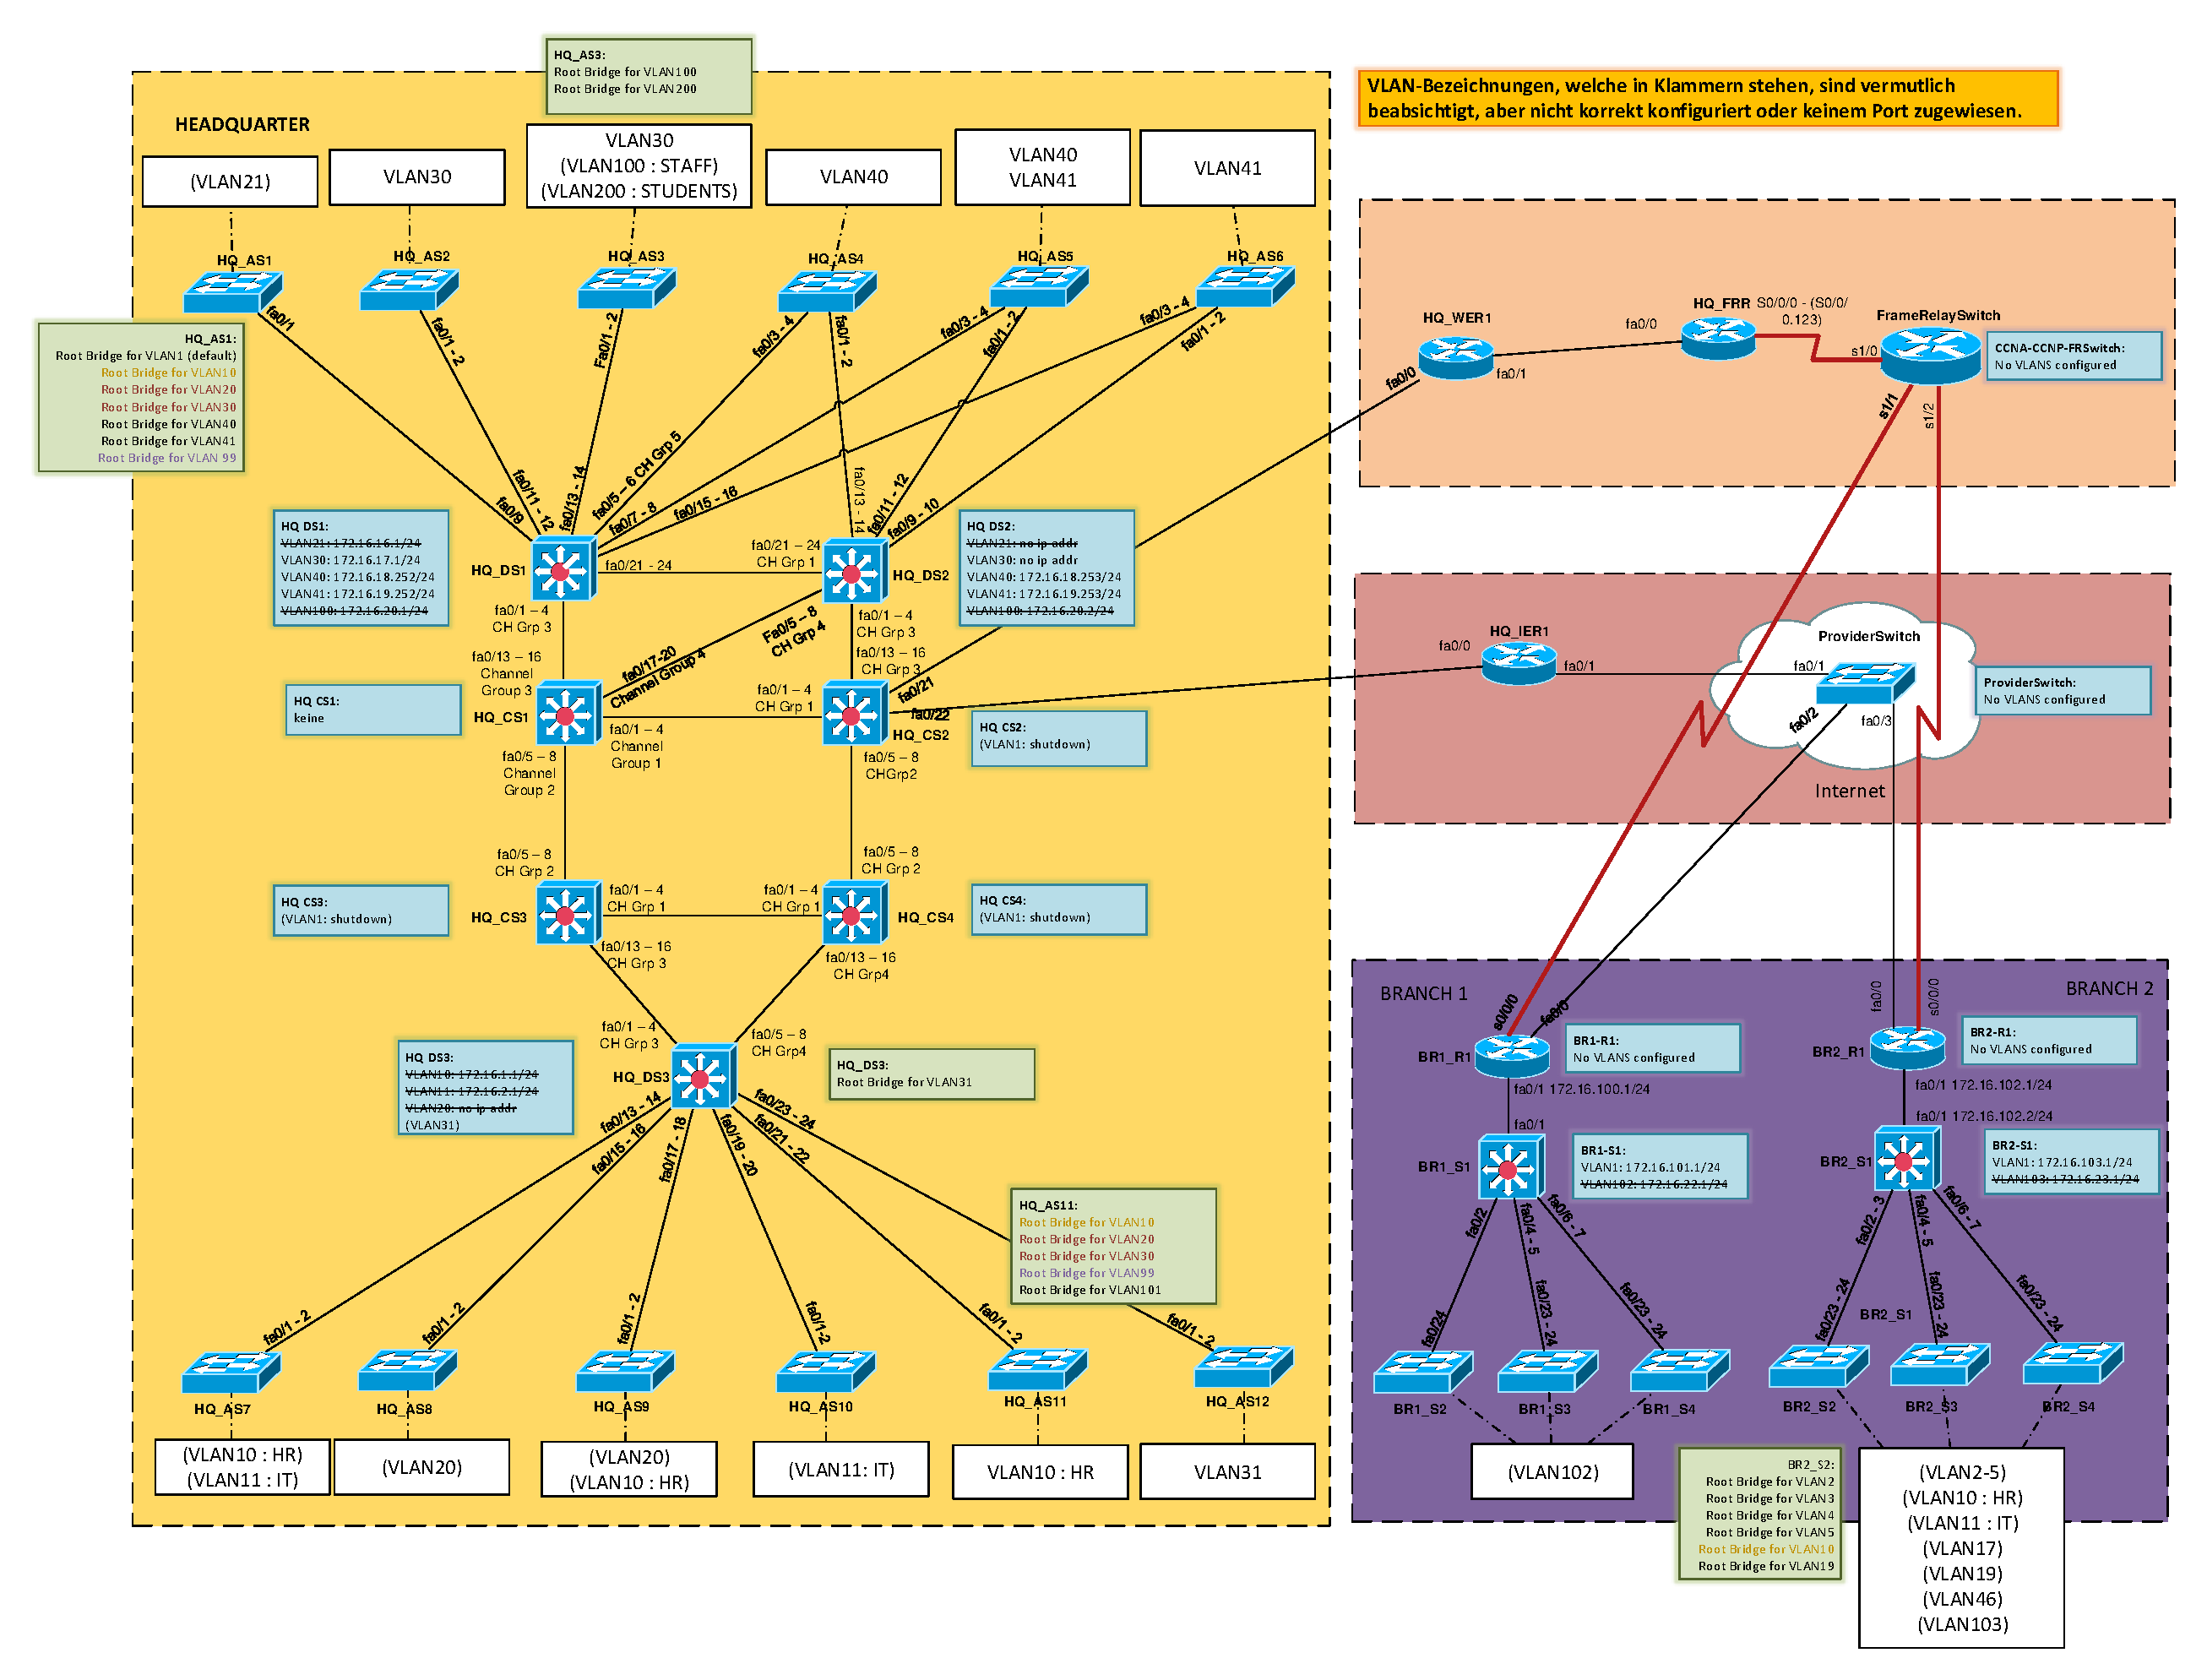
\includepdf[pages={1},landscape=true]{appendix/schemes/vlan.pdf}
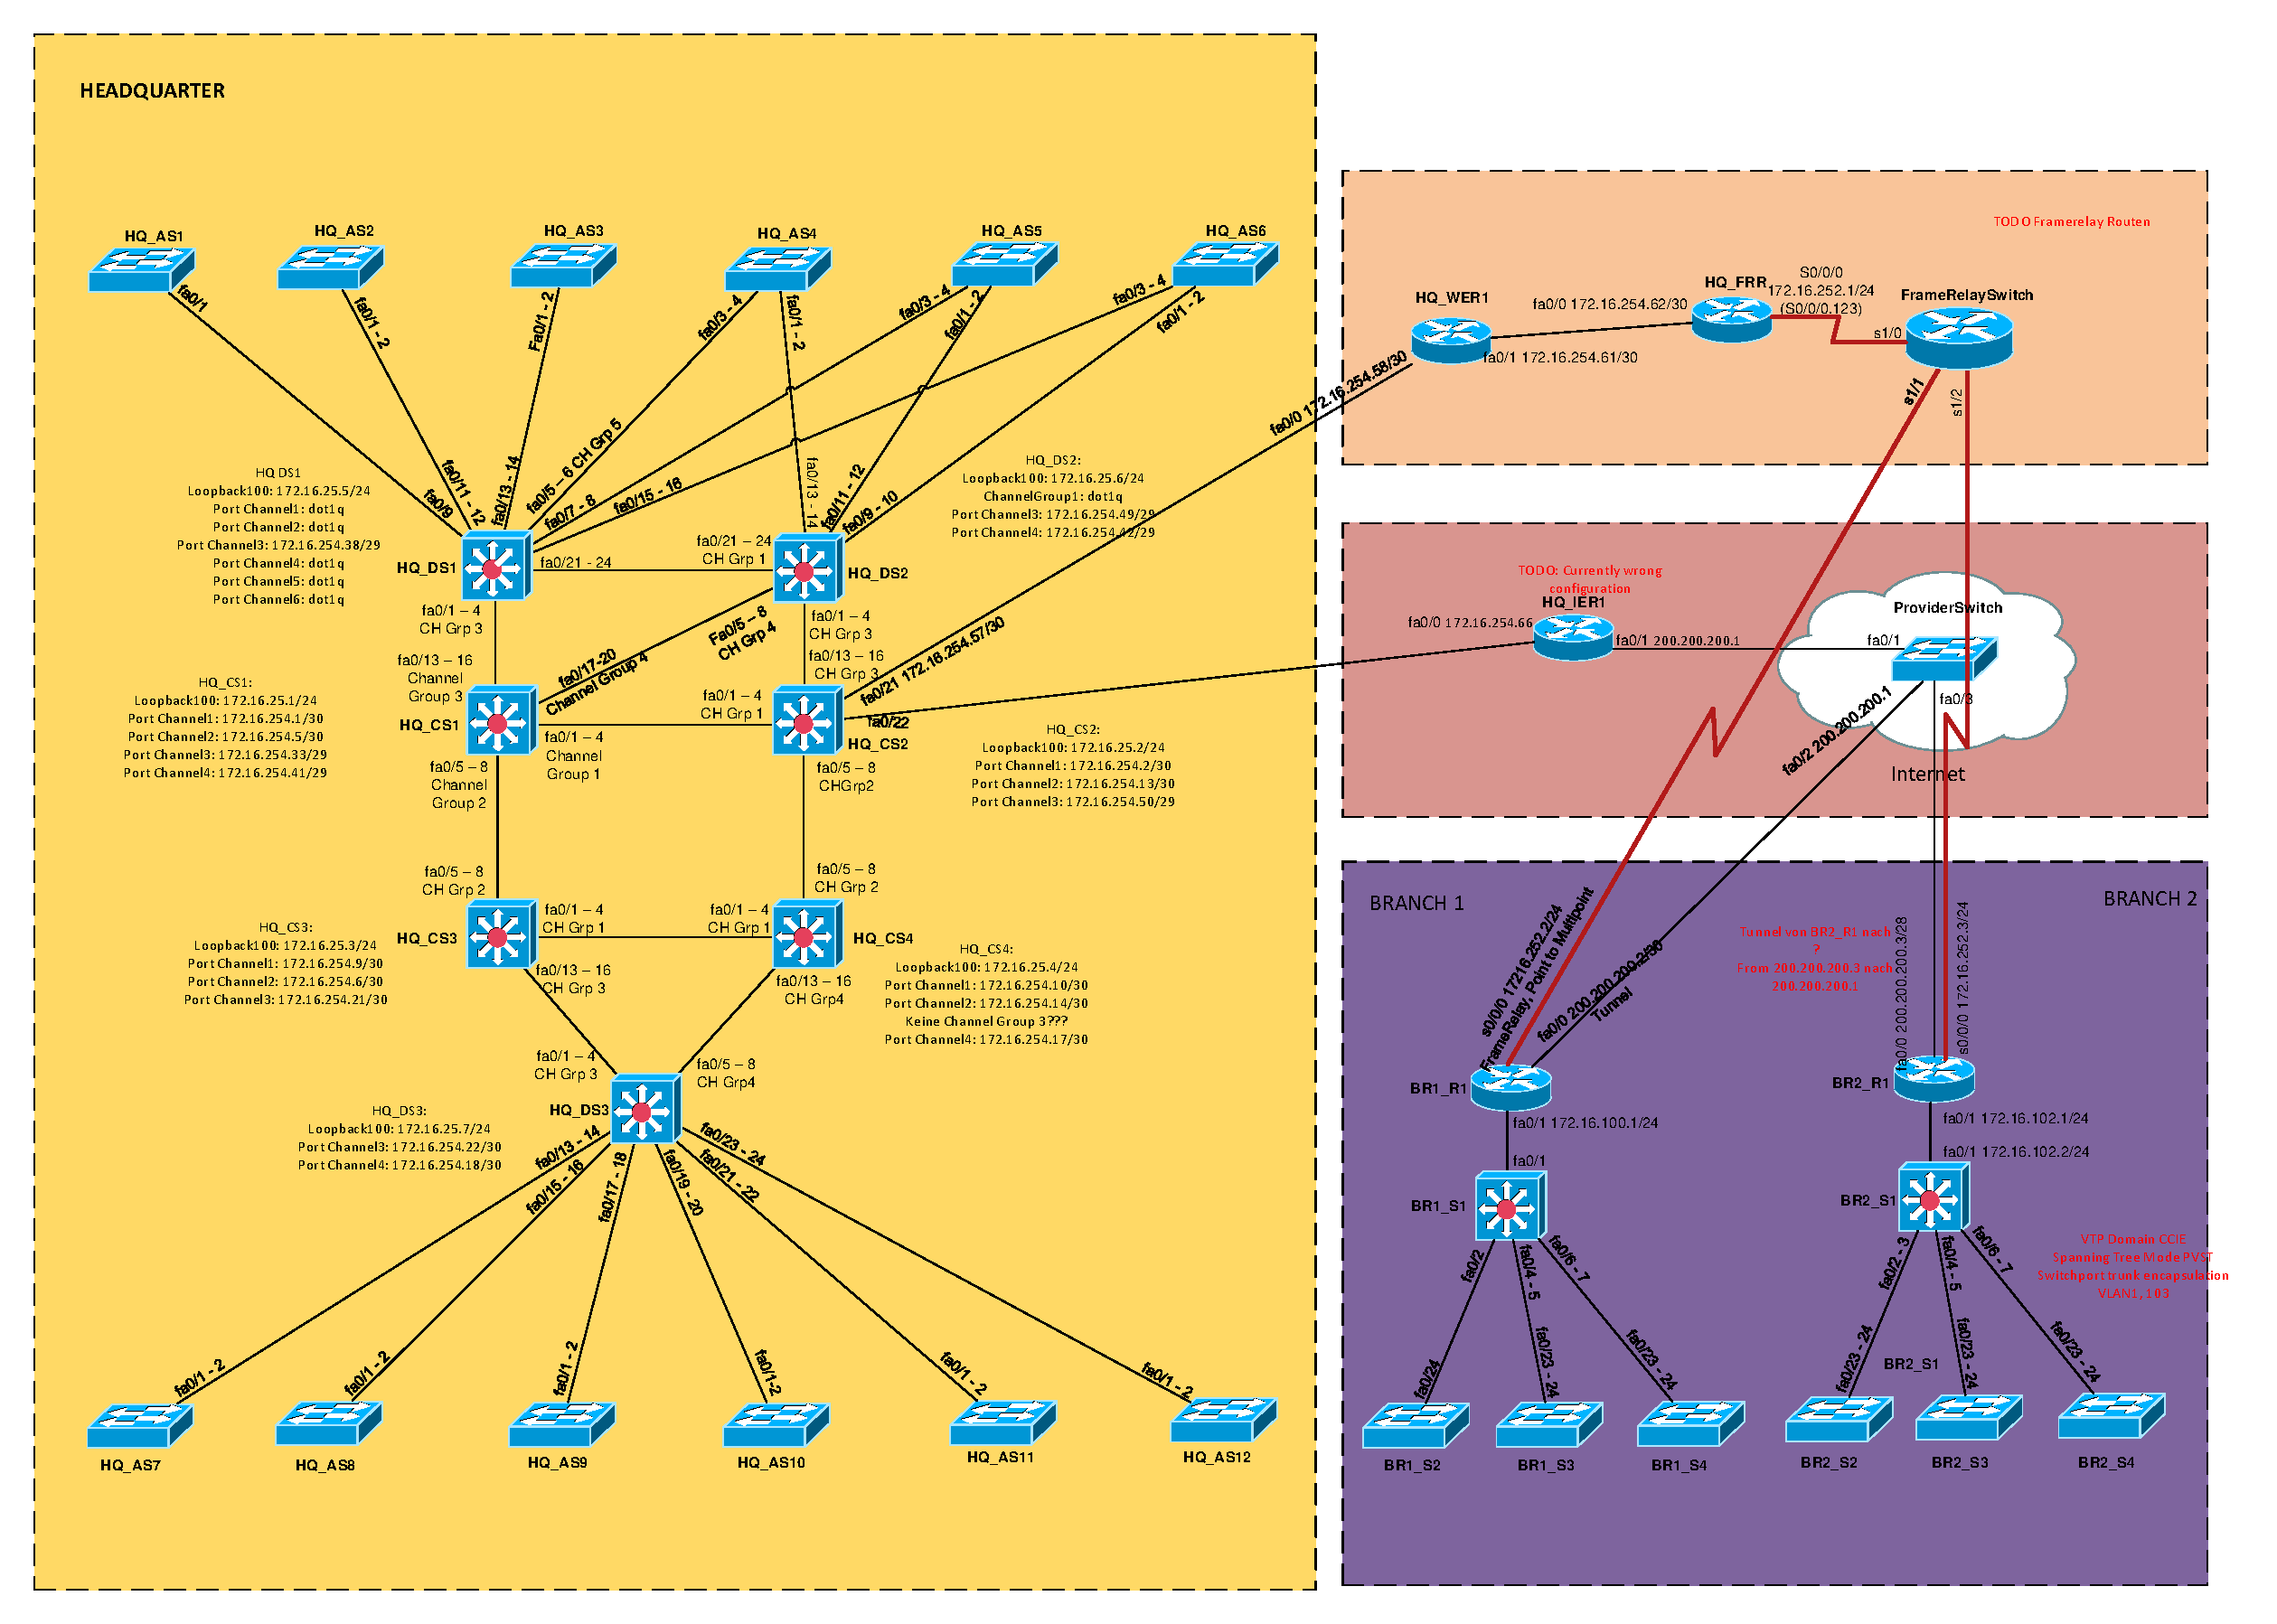
\includepdf[pages={1},landscape=true]{appendix/schemes/L1.pdf}


\section{Gefundene Fehler und Verbesserungsvorschläge}


\subsection{Allgemeine Verbesserungsvorschläge}

\begin{itemize}
	\item Auf allen Routern sollte der DNS-Lookup bei einem Tippfehler deaktiviert werden, um die Administration zu vereinfachen.
	\item Die Geräte z.B. Switches in den Branches und Headquarter sind inkonsistent benannt.
	\item Der DHCP Pool für das VLAN 11 (IT) wurde nicht gleich wie das VLAN benannt
\end{itemize}

\subsection{Layer 1}
Auf Layer 1 (dem physischen Netzwerk) gibt es gemäss der Vorgabe dieses Reports keine Fehler.

\subsection{Layer 2}
\subsubsection{Design}
\begin{itemize}
	\item HQ\_CS2 bildet die einzige Verbindung zu den Branches. Es bildet somit einen Single Point of Failure.
\end{itemize}

\subsubsection{Ethernet}

\begin{description}
	\item[HQ\_DS2] \hfill \\
	  \begin{itemize}
	    \item Der HQ\_DS2 hat eine andere MTU als alle anderen Switches und Router, dadurch kommt es zu Fehlern.
	    \item Der Port Fa0/21 bei HQ\_DS2 hat den Status \lstinline|err-disabled|
	    \item Die Port Channel Group 1 bei HQ\_DS2 hat den Status \lstinline|err-disabled|
          \end{itemize}
	\item[HQ\_CS1] \hfill \\
		\begin{itemize}
			\item Die Verbindung zu HQ\_DS1 ist als bandwidth 10000 und speed 10 eingerichtet.
			\item Die Verbindung zu HQ\_DS2 ist als half duplex, speed 100 und bandwidth 10000 eingerichtet.
		\end{itemize}
	\item[HQ\_CS2] \hfill \\
	 Der HQ\_CS2 hat zum HQ\_CS4 eine Netzwerkverbindung mit bandwidth 10000 und speed 10 konfiguriert.
	\item[HQ\_CS4] \hfill \\
		Die Port Channel Group 1 bei HQ\_CS4 ist auf 10Mbit/s eingestellt. 
	\item[HQ\_AS6] \hfill \\
		Die Port Channel Group 6 bei HQ\_AS6 ist auf 10Mbit/s eingestellt. Zusätzlich haben sie den Status \lstinline|err-disabled|
\end{description}

\subsubsection{Spanning Tree}

Beim Spanning Tree ist HQ\_AS1 als Root in diversen VLAN's eingetragen, dies ist jedoch eher eine Suboptimale Wahl, da so unnötig Traffic über die Verbindung zu DS1 gespielt wird.

%TODO: Genauer anschauen bei anderen Geräten.

In der folgenden Sektion VLAN sind noch einige als Fastport eingestellte Ports vermerkt, diese können auch den Spanning Tree beeinflussen.

\subsubsection{VLAN}
\begin{description}
% Headquarter
	\item[HQ\_AS1] \hfill \\
	  \begin{itemize}
		  \item VLAN1 ist Administratively Down
		  \item Nur Fa0/2, Gi0/1, Gi0/2 sind auf HQ\_AS1 für VLAN1 konfiguriert
		  \item Die meisten Interfaces auf HQ\_AS1 sind im VLAN 21; dies ist in  der VLAN Konfiguration nicht eingerichtet.
		  \item Fa0/1 ist nicht auf trunk konfiguriert, damit funktioniert der Upstream nicht.
	  \end{itemize}
	\item[HQ\_AS4] \hfill \\
	 Auf den meisten Trunkports ist portfast eingestellt, dies kann zu Problemen mit SPF / Switching Loops führen.
	\item[HQ\_AS6] \hfill \\
	 Die Link-Gruppe 6 des Uplink ist als shutdown eingestellt, deshalb hat der Switch keinen Uplink.
	\item[HQ\_AS7] \hfill \\
	 Beim HQ\_AS7 sind VLAN 10 und 11 auf Ports eingerichtet, aber nicht in der VLAN-Konfiguration
	\item[HQ\_AS3] \hfill 
	\begin{itemize}
		\item Beim HQ\_AS3 sind VLAN 100 und 200 auf Ports eingerichtet, aber nicht in der VLAN-Konfiguration.
	\end{itemize}
	\item[HQ\_AS8] \hfill \\
	 Beim HQ\_AS8 ist VLAN 20 auf Ports eingerichtet, aber nicht in der VLAN-Konfiguration.
	\item[HQ\_AS9] \hfill \\
	 Beim HQ\_AS9 VLAN 10 und VLAN 20 auf Ports eingerichtet, aber nicht in der VLAN-Konfiguration.
	\item[HQ\_AS10] \hfill \\
	 Beim HQ\_AS10 VLAN 11 auf Ports eingerichtet, aber nicht in der VLAN-Konfiguration.
	\item[HQ\_DS3] \hfill \\
	 Die VLANs auf HQ\_DS3 sind down, daher haben HQ\_AS7 bis HQ\_AS12 kein Netzwerkzugriff.
% Filialen
	\item[BR1\_S2] \hfill \\
	  \begin{itemize} 
		  \item Die VLANs nicht auf den Ports zugeordnet.
		  \item Die Trunk-Ports zum Router sind nicht richtig konfiguriert (nämlich auf access und spanning-tree portfast)
	  \end{itemize}
	\item[BR1\_S3] \hfill \\
	  \begin{itemize} 
		  \item Die VLANs nicht auf den Ports zugeordnet. 
		  \item Die Trunk-Ports zum Router sind nicht richtig konfiguriert (nämlich auf access und spanning-tree portfast)
	  \end{itemize}
	\item[BR1\_S4] \hfill \\
	  \begin{itemize} 
		  \item Die VLANs nicht auf den Ports zugeordnet. 
		  \item Die Trunk-Ports zum Router sind nicht richtig konfiguriert (nämlich auf access und spanning-tree portfast)
	  \end{itemize}
	\item[BR2\_S1] \hfill \\
		\begin{itemize}
			\item VLAN1 ist shutdown, darum gehen die Access-Switches im ganzen BR2 nicht.
		\end{itemize}
	\item[BR2\_S2] \hfill \\
	  \begin{itemize}
		  \item Die VLANs nicht auf den Ports zugeordnet.
		  \item VLAN103 ist als Virtuelles Interface eingerichtet, allerdings nicht in der vlan.dat eingetragen.
		  \item Die Trunk-Ports zum Router sind nicht richtig konfiguriert (nämlich auf access und spanning-tree portfast beim Fa23 sowie trunk auf Fa24 ohne grouping.)
		\end{itemize}
	\item[BR2\_S3] \hfill \\
	  \begin{itemize}
	  	\item Die VLANs nicht auf den Ports zugeordnet.
		  \item VLAN103 ist als Virtuelles Interface eingerichtet, allerdings nicht in der vlan.dat eingetragen.
		  \item Port Fa23 und Fa24 sind auf access-port und portfast konfiguriert statt auf trunk.
		\end{itemize}
	\item[BR2\_S4] \hfill \\
	  \begin{itemize}
	  	\item Die VLANs nicht auf den Ports zugeordnet.
		  \item VLAN103 ist als Virtuelles Interface eingerichtet, allerdings nicht in der vlan.dat eingetragen.
		\end{itemize}
\end{description}

\subsubsection{Frame Relay}

\begin{description}
	\item[FrameRelaySwitch] \hfill \\
	 Auf der Netzwerktopologie wird am FrameRelaySwitch Port S1/2 zum BR2\_R1 benutzt, allerdings ist die Verkabung auf Port S1/3. Die Konfiguration scheint allerdings trotzdem korrekt zu sein.
\end{description}

\subsection{Layer 3}

Sehr wahrscheinlich bestehen noch mehr Fehler auf Layer 3 als hier vermerkt, diese konnten allerdings aufgrund \textbf{fataler} Probleme auf Layer 2 nicht getestet werden.

\subsubsection{Routen}
%TODO Michi Routen erklärung: Warum 1x über FRR und 1x über Router!!!!!
\begin{description}
	\item[HQ\_DS1] \hfill \\
	 Beim HQ\_DS1 ist die Verbindung zu HQ\_DS2 inaktiv, weil die Channel Group 1 keine IP zugeordnet hat.
	 \item[BR1\_R1 und BR2\_R2] hier sind unterschiedliche Netzmasken für 200.200.200.0 eingetragen.
\end{description}

\subsubsection{Routen / OSPF}

\begin{description}
	\item[FrameRelayRouter] \hfill \\
		\begin{itemize}
			\item Die Routen über das FrameRelay sind überall sehr hoch. Ist dies bewusst aufgrund der Kosten gewählt?
			\item Das Framerealy hat ab ca. 6300 Bytes/s starken Paketverlust (Anfragen vereinbarte Dienstleistung mit ISP)
		\end{itemize}
	\item[Routing Branches] \hfill \\
		Das Routing zu den Branches ist inkonsistent. Eventuell besteht ein Problem bei den Internet / WAN-Verbindungen. Dies muss in weiteren Abklärungen festgestellt werden.
\end{description}

%TODO: nächsten Abschnitt löschen?
\section{Messungen}
Alle Durchgeführten Messungen sind im Anhang \ref{appendix:measures} zu finden.

\section{Folgerungen}
Während der, sich als sehr aufwändig gestaltenden, Analyse, sind uns viele Fehlkonfigurationen und Unschönheiten aufgefallen. Diese gilt es nun in einem letzten Schritt zu beheben. Die Korrektur der erkannten Fehler ist im Abschnitt \ref{sec:recommedations} beschrieben, wobei wir auf eine Lösung möglichst kleinem Einfluss auf das produktive System geachtet haben. Zusätzlich versuchten diese Punkte zu ändern, bei denen möglichst wenig Kosten anfallen würden.

\subsection{Empfehlungen}
\label{sec:recommedations}
Aufgrund der vorangehenden Erkenntnissen empfehlen wir, an folgenden Punkten anzusetzen:
%TODO add recommedations
\begin{enumerate}
	\item Alle 10 und 100Mbit/s Leitung auf den maximal physisch möglichen Durchsatz aufschrauben.
\end{enumerate}

\subsection{Kostenvoranschlag}
Für die Umsetzung unserer Empfehlungen würden folgende Kosten anfallen.
\begin{table}[h]
	\centering
	\begin{tabu} to \linewidth {X[3] X X X}
		\toprule 
		Beschreibung & Zeitaufwand in h  & Stundenansatz in CHF & Total \\
		\midrule
		VLAN Konsistenz erstellen & 8 & 150 & 1200 \\
		Linkgeschwindigkeiten und Duplexmodus anpassen & 1 & 150 & 150 \\
		Zusätzliche Anbindung der Branches über HQ\_CS4 & 6 & 150 & 900 \\
		
		\textbf{Total} & & & \underline{\underline{2250 CHF}} \\
		\bottomrule 
	\end{tabu} 
	\caption{Kostenvoranschlag}
\end{table}

\appendix

\section{Konfigurationen}
\label{appendix:configurations}

\subsection{BR1-R1}
\subsubsection{Running Configuration}
\lstinputlisting{appendix/config/br1-r1/br1-r1-config.txt}

\subsubsection{IP Interfaces}
\lstinputlisting{appendix/config/br1-r1/br1-r1-interface.txt}

\subsubsection{Interface Status}
\lstinputlisting{appendix/config/br1-r1/br1-r1-status.txt}

\subsubsection{Neighbors}
\lstinputlisting{appendix/config/br1-r1/br1-r1-neighbors.txt}

\subsection{BR2-R1}
\subsubsection{Running Configuration}
\lstinputlisting{appendix/config/br2-r1/br2-ri-config.txt}

\subsubsection{IP Interfaces}
\lstinputlisting{appendix/config/br2-r1/br2-ri-interface.txt}

\subsubsection{Interface Status}
\lstinputlisting{appendix/config/br2-r1/br2-ri-status.txt}

\subsubsection{Neighbors}
\lstinputlisting{appendix/config/br2-r1/br2-ri-neighbors.txt}

\subsection{BR2-S1}
\subsubsection{Running Configuration}
\lstinputlisting{appendix/config/br2-s1/br2-s1-config.txt}

\subsubsection{IP Interfaces}
\lstinputlisting{appendix/config/br2-s1/br2-s1-interface.txt}

\subsubsection{Interface Status}
\lstinputlisting{appendix/config/br2-s1/br2-s1-status.txt}

\subsubsection{Neighbors}
\lstinputlisting{appendix/config/br2-s1/br2-s1-neighbors.txt}

\subsection{CCNA-CCNP-FRSwitch}
\subsubsection{Running Configuration}
\lstinputlisting{appendix/config/framerelayswitch/framerelayswitch-config.txt}

\subsubsection{IP Interfaces}
\lstinputlisting{appendix/config/framerelayswitch/framerelayswitch-interface.txt}

\subsubsection{Interface Status}
\lstinputlisting{appendix/config/framerelayswitch/framerelayswitch-status.txt}

\subsubsection{Neighbors}
\lstinputlisting{appendix/config/framerelayswitch/framerelayswitch-neighbors.txt}

\subsection{HQ FrameRelay Router (HQ-FRR)}
\subsubsection{Running Configuration}
\lstinputlisting{appendix/config/hq-frr/hq-frr-config.txt}

\subsubsection{IP Interfaces}
\lstinputlisting{appendix/config/hq-frr/hq-frr-interface.txt}

\subsubsection{Interface Status}
\lstinputlisting{appendix/config/hq-frr/hq-frr-status.txt}

\subsubsection{Neighbors}
\lstinputlisting{appendix/config/hq-frr/hq-frr-neighbors.txt}

\subsection{HQ-IER1}
\subsubsection{Running Configuration}
\lstinputlisting{appendix/config/hq-ier1/hq-ier1-config.txt}

\subsubsection{IP Interfaces}
\lstinputlisting{appendix/config/hq-ier1/hq-ier1-interface.txt}

\subsubsection{Interface Status}
\lstinputlisting{appendix/config/hq-ier1/hq-ier1-status.txt}

\subsubsection{Neighbors}
\lstinputlisting{appendix/config/hq-ier1/hq-ier1-neighbors.txt}

\subsection{HQ-WER1}
\subsubsection{Running Configuration}
\lstinputlisting{appendix/config/hq-wer1/hq-wer1-config.txt}

\subsubsection{IP Interfaces}
\lstinputlisting{appendix/config/hq-wer1/hq-wer1-interface.txt}

\subsubsection{Interface Status}
\lstinputlisting{appendix/config/hq-wer1/hq-wer1-status.txt}

\subsubsection{Neighbors}
\lstinputlisting{appendix/config/hq-wer1/hq-wer1-neighbors.txt}

\subsection{HQ CS1}
\subsubsection{Running Configuration}
\lstinputlisting{appendix/config/hq-cs1/hq-cs1-config.txt}

\subsubsection{IP Interfaces}
\lstinputlisting{appendix/config/hq-cs1/hq-cs1-interface.txt}

\subsubsection{Interface Status}
\lstinputlisting{appendix/config/hq-cs1/hq-cs1-status.txt}

\subsubsection{Neighbors}
\lstinputlisting{appendix/config/hq-cs1/hq-cs1-neighbors.txt}

\subsection{HQ CS2}
\subsubsection{Running Configuration}
\lstinputlisting{appendix/config/hq-cs2/hq-cs2-config.txt}

\subsubsection{IP Interfaces}
\lstinputlisting{appendix/config/hq-cs2/hq-cs2-interface.txt}

\subsubsection{Interface Status}
\lstinputlisting{appendix/config/hq-cs2/hq-cs2-status.txt}

\subsubsection{Neighbors}
\lstinputlisting{appendix/config/hq-cs2/hq-cs2-neighbors.txt}

\subsection{HQ CS3}
\subsubsection{Running Configuration}
\lstinputlisting{appendix/config/hq-cs3/hq-cs3-config.txt}

\subsubsection{IP Interfaces}
\lstinputlisting{appendix/config/hq-cs3/hq-cs3-interface.txt}

\subsubsection{Interface Status}
\lstinputlisting{appendix/config/hq-cs3/hq-cs3-status.txt}

\subsubsection{Neighbors}
\lstinputlisting{appendix/config/hq-cs3/hq-cs3-neighbors.txt}

\subsection{HQ CS4}
\subsubsection{Running Configuration}
\lstinputlisting{appendix/config/hq-cs4/hq-cs4-config.txt}

\subsubsection{IP Interfaces}
\lstinputlisting{appendix/config/hq-cs4/hq-cs4-interface.txt}

\subsubsection{Interface Status}
\lstinputlisting{appendix/config/hq-cs4/hq-cs4-status.txt}

\subsubsection{Neighbors}
\lstinputlisting{appendix/config/hq-cs4/hq-cs4-neighbors.txt}

\subsection{HQ DS1}
\subsubsection{Running Configuration}
\lstinputlisting{appendix/config/hq-ds1/hq-ds1-config.txt}

\subsubsection{IP Interfaces}
\lstinputlisting{appendix/config/hq-ds1/hq-ds1-interface.txt}

\subsubsection{Interface Status}
\lstinputlisting{appendix/config/hq-ds1/hq-ds1-status.txt}

\subsubsection{Neighbors}
\lstinputlisting{appendix/config/hq-ds1/hq-ds1-neighbors.txt}

\subsection{HQ DS2}
\subsubsection{Running Configuration}
\lstinputlisting{appendix/config/hq-ds2/hq-ds2-config.txt}

\subsubsection{IP Interfaces}
\lstinputlisting{appendix/config/hq-ds2/hq-ds2-interface.txt}

\subsubsection{Interface Status}
\lstinputlisting{appendix/config/hq-ds2/hq-ds2-status.txt}

\subsubsection{Neighbors}
\lstinputlisting{appendix/config/hq-ds2/hq-ds2-neighbors.txt}

\subsection{HQ DS3}
\subsubsection{Running Configuration}
\lstinputlisting{appendix/config/hq-ds3/hq-ds3-config.txt}

\subsubsection{IP Interfaces}
\lstinputlisting{appendix/config/hq-ds3/hq-ds3-interface.txt}

\subsubsection{Interface Status}
\lstinputlisting{appendix/config/hq-ds3/hq-ds3-status.txt}

\subsubsection{Neighbors}
\lstinputlisting{appendix/config/hq-ds3/hq-ds3-neighbors.txt}


\section{Messungen}
\label{appendix:measures}
\subsection{Von X nach Y}
\lstinputlisting{appendix/config/br2-r1/br2-ri-config.txt}

% Code Listings
% \lstlistoflistings

% List of figures
% \listoffigures

% List of tables
% \listoftables

% Bibliography
% \bibliographystyle{plain} 
% \bibliography{literatur}

\end{document}
